%% The following is a directive for TeXShop to indicate the main file
%%!TEX root = diss.tex

\chapter{Fast Simulation}
\label{ch:Methods}
To run particle identification on each event, a fast simulation of the optical photon distributions in the EMPHATIC ARICH detector was developed.
The simulation of the ARICH detector was created using \textsc{ROOT}: an object-oriented scientific computing framework based off C++ and developed at CERN \cite{root}.
\textsc{ROOT} is used for its ease of use, the high degree of organization and extensibility that comes from its object-oriented nature, and its high efficiency when compiled.
The simulation was created in steps of increasing added complexity, which are outlined in this chapter. \TODO{remove this sentence}


\section{Initial Simulation}
\label{sec:experiment}
The first step in building the simulation was to generate a stream of particles, representing the charged pions and kaons and protons produced in an experiment.
If we define the $z$ axis to be the downstream direction, then the inputs to the simulation are:
\begin{itemize}
\item the initial $x$ and $y$ position of a particle at $z=0$,
\item the error on the $x$ and $y$ position of the particle, corresponding to the position resolution of the upstream particle tracker,
\item the $x$ and $y$ components of the unit vector representing the direction of the particle's movement,
\item the error on the $x$ and $y$ direction of the particle, corresponding to the direction resolution of the upstream particle tracker, and
\item the velocity $\beta$ of the particle.
\end{itemize} 
The simulation generates 10,000 such particles whose initial positions and directions are randomly drawn from a Gaussian distribution with the specified mean values and errors.

A layer of aerogel was defined in the simulation as a 2 cm thick, 10 cm by 10 cm volume, with a refractive index of 1.035, placed with its back edge at $z=0$.
For each simulated particle with a given velocity $\beta$, we use equation \ref{eq:photonNumber} to calculate the mean number of photons emitted per unit length, and generate a number of photons equal to this value multiplied by the distance the particle has to travel through the aerogel.
The initial position of these photons are randomly distributed along the path travelled by the particle through the aerogel.
Their polar angle $\theta$ with respect to the direction of travel of the particle is given by equation \ref{eq:cherenkovAngle}, and their azimuthal angle is randomly drawn from between 0 and $2\pi$.
If we are given the direction vector of the particle, we can use a rotation matrix to get the resulting direction vectors for each of the photons it generates.
This is given by \TODO{Include here Rodrigue's rotation formula, and how it is adapted into matrix form}.

The photons ultimately are detected by an array of PMTs, which have a known quantum efficiency, characterized over a range of frequencies of light.
The efficiency curve of the PMTs is plotted in Figure \ref{fig:qEff} and is given over a range from 267 to 687 nm  \cite{H12700} .

\begin{figure}[]
\centering
\resizebox{0.9\textwidth}{!}{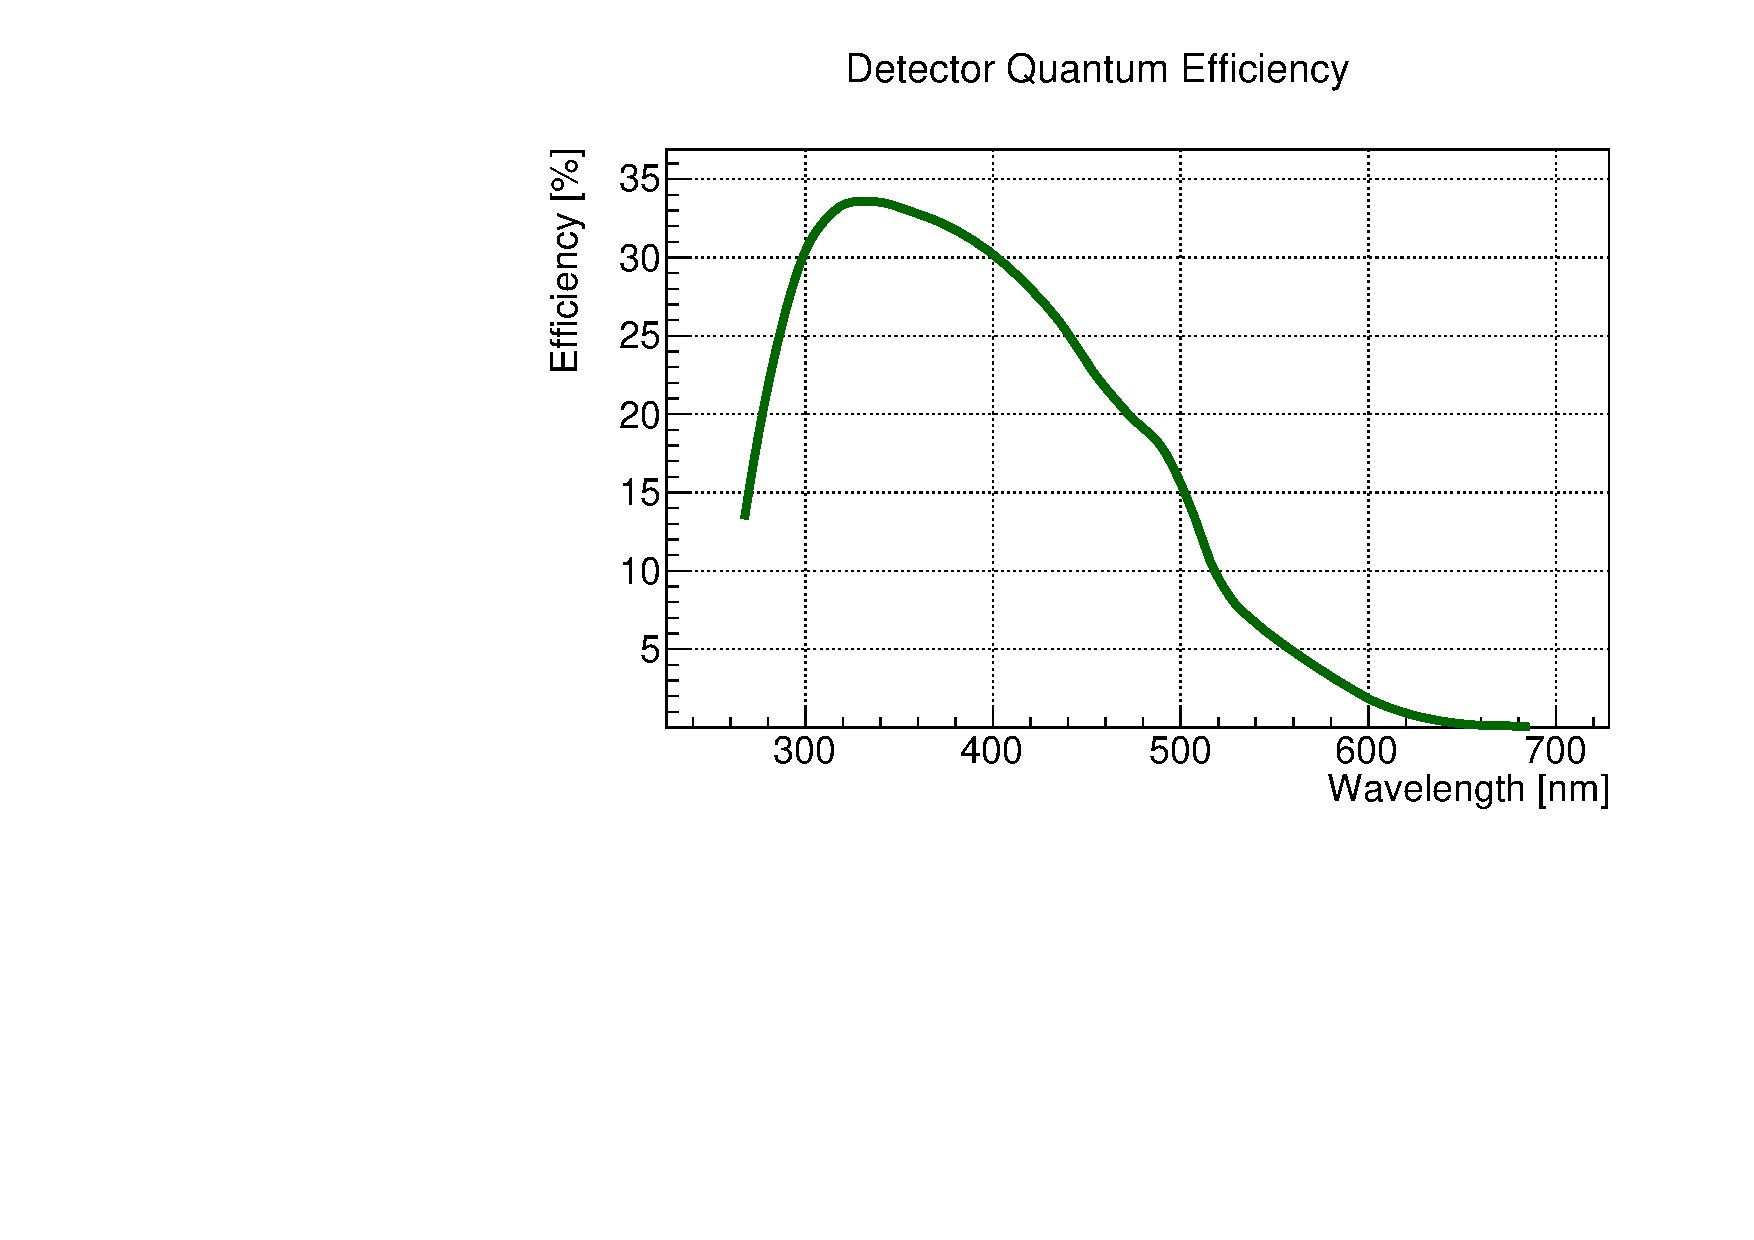
\includegraphics{./figs/qEff.pdf}}
\caption[Quantum Efficiency of H12700 PMT used by EMPHATIC.]{Quantum Efficiency of H12700 PMT used by EMPHATIC.}
\label{fig:qEff} 
\end{figure}

From equation \ref{eq:frankTamm}, we see that the distribution of photon wavelengths follows a distribution proportional to $1/\lambda^2$, so each photon is produced with a wavelength randomly drawn from this distribution on a range from 250 nm to 695 nm.
If we linearly extrapolate the quantum efficiency curve, we see that we do not expect to get any detector response for photons of wavelengths outside of this range of wavelengths.
Because all optical processes included in this simulation are inelastic, we do not expect any photon wavelength to change between the point of generation and the point of detection.
Therefore, after generating Cherenkov photons we may randomly reject them immediately based on their eventual probability of being detected by the PMTs, and not simulate their paths any further if we decide that they would not be detected. \TODO{reword}

The PMTs have dimensions of 48.5 mm $\times$ 48.5 mm.
Each PMT contains $8 \times 8$ pixels, and have a packing density of 87\%. 
The PMTs are expected to be arranged onto a 30 cm $\times$ 30 cm plane with a packing efficiency of $80\%$, 20 cm downstream of the first layer of aerogel.
To model the photon detector array, we simply project the photons downstream onto a 30 cm $\times$ 30 cm histogram with $48 \times 48$ bins.
The number of photons counted in each bin is scaled by a factor of $80\% \times 87\%$ to account for the packing efficiencies.

Two examples of photon distribution arising from this simple simulation are shown in Figure \ref{fig:noScat}. While this simulation well approximates the expected location of a particle's photon rings for a single layer of aerogel, it is missing a number of key effects that would allow it to actually be used to calculate a realistic photon distribution.


\begin{figure}[]
  \centering
  \subfloat[Centered beam.]{\includegraphics[width=0.45\textwidth]{./figs/noscatter.pdf}\label{fig:f1}}
  \hfill
  \subfloat[Beam at an angle of 0.44 radians off the $z$-axis]{\includegraphics[width=0.45\textwidth]{./figs/noscatterangle.pdf}\label{fig:f2}}
  \caption{ Examples of two photon distributions, showing the mean number of photons we would expect to detect in each PMT pixel, after accounting for detector efficiency, but ignoring any optical effects. \TODO{Redo these two figures - make them the same dimension, and tall so that they can be placed side by side}}
  \label{fig:noScat}
\end{figure}

\section{Optical Effects}
Following this initial simulation, more sophisticated optical effects were added in. 

\subsection{Rayleigh Scattering}
The properties of each of the 2 cm thick layers of aerogel available to the EMPHATIC experiment were characterized by another member of the collaboration \cite{aerogelTabata}: their refractive indices were measured for light with a wavelength of 405 nm, and the transmittances of light were measured for light of wavelengths ranging from 190 nm to 800 nm.
The transmittance and refractive index of each aerogel are shown in Figure \ref{fig:transmittance}.

\begin{figure}[]
  \centering
  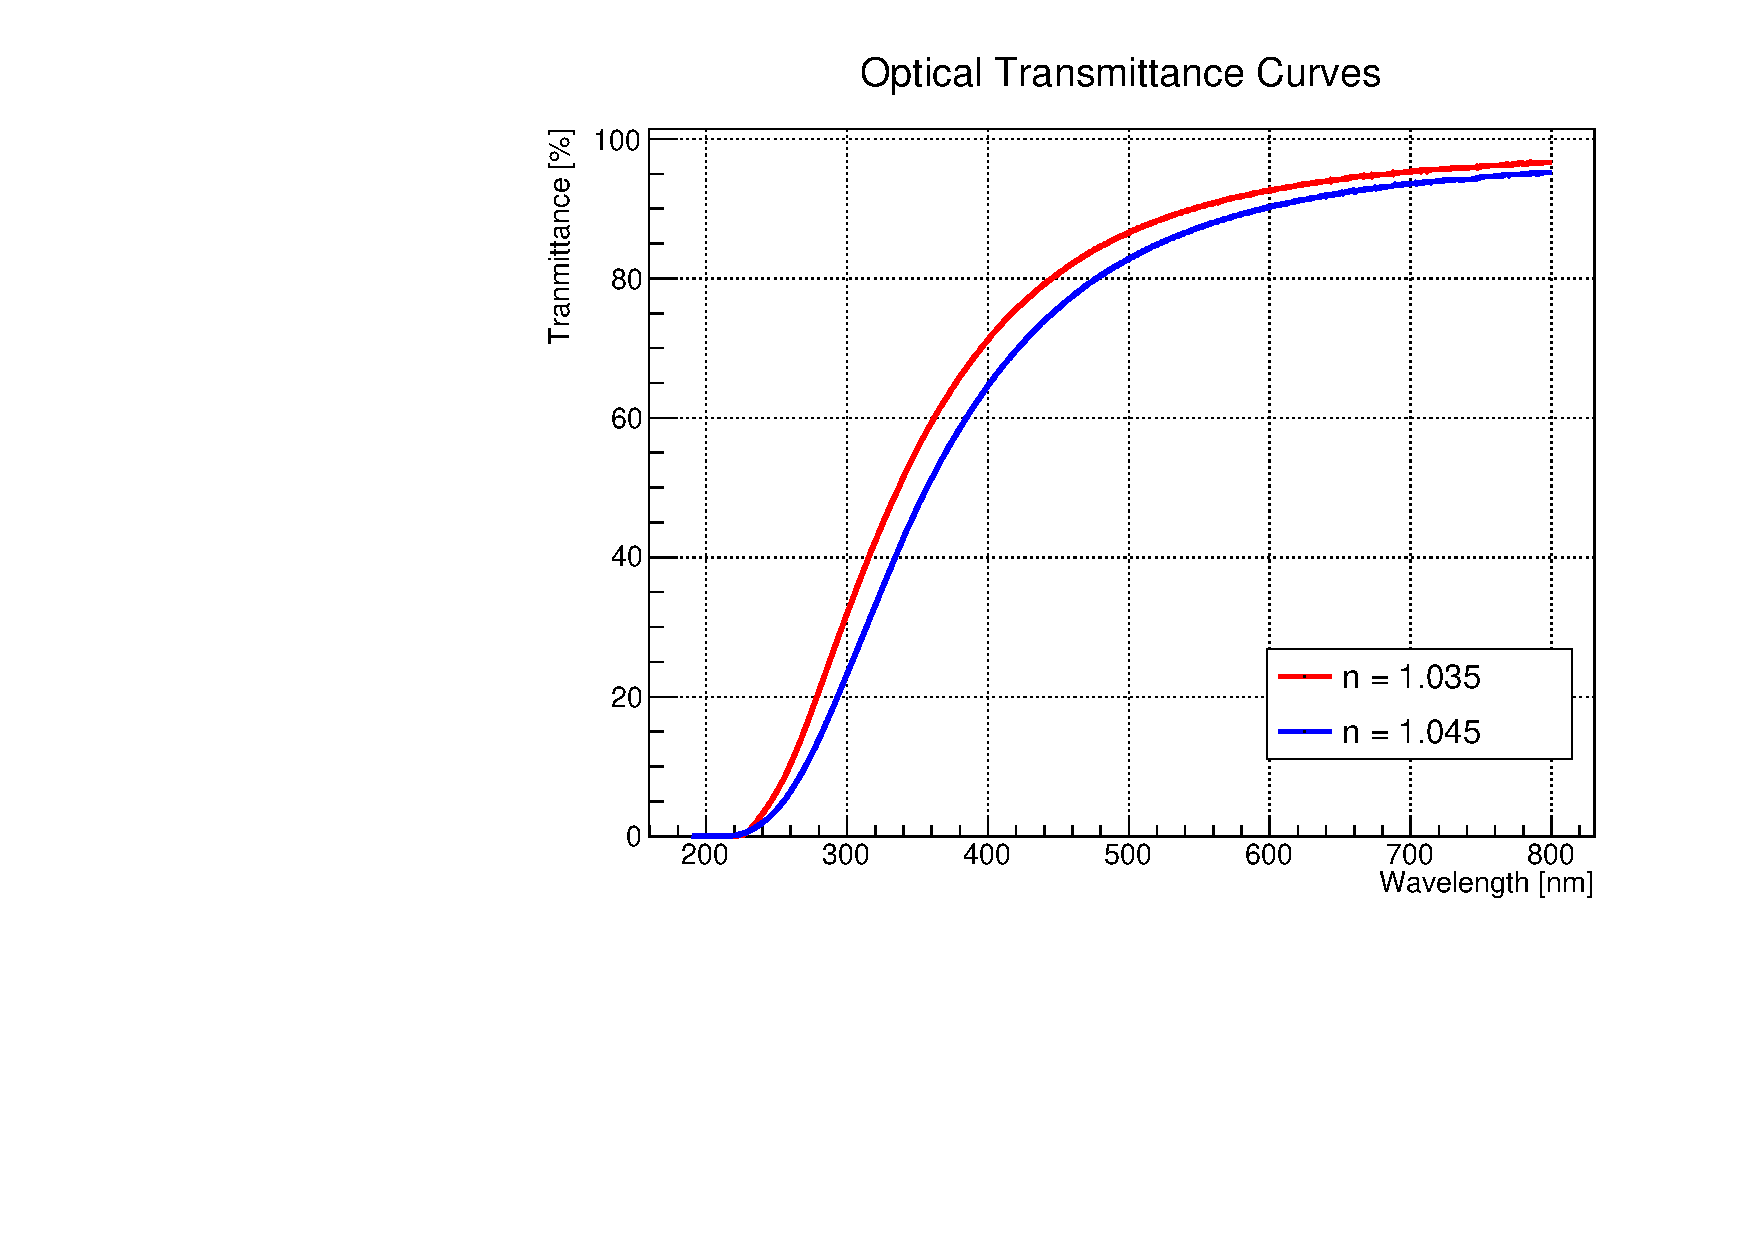
\includegraphics[width=0.9\textwidth]{./figs/transmittance.pdf}
    \caption{Optical transmittance curves of aerogels with n = 1.035 and n = 1.045.}
  \label{fig:transmittance}
\end{figure}

As described in Section \ref{sec:optics}, the primary optical effect to account for is Rayleigh Scattering, wherein photons scatter with a probability proportional to $\lambda^{-4}$, and in a direction proportional to $1 + \cos^2(\theta)$.
If we assume that the transmittance of light through the aerogels is only affected by Rayleigh scattering then we can approximate $L(\lambda)$, the Rayleigh scattering interaction length at each wavelength, with the following formula:

\begin{equation}
L(\lambda) = \frac{-d}{\log(T(\lambda))}
    \label{eq:scatLength}
\end{equation}

In this equation, $T(\lambda)$ is the transmittance of light at a wavelength $\lambda$ across some thickness $d$ of the aerogel.
In order to efficiently sample a random distance before scattering, we can apply inverse transform sampling \TODO{Cite inverse transform sampling}.
The probability $p$ that a photon has scattered after travelling some distance $x$ through the aerogel is given by

\begin{equation}
p = 1 - \exp(-x/L)
    \label{eq:scatProb}
\end{equation}

To randomly draw a distance $x$ from this distribution, we can sample some $p$ uniformly on the range $[0,1]$, and get a distance $x$ by calculating the inverse:

\begin{equation}
x =   -L\ln(1-p)
  \label{eq:randomScat}
\end{equation}

In the simulation, when each photon is generated, a random ``distance until scattering" is calculated this way. 
We check whether or not a photon would still be in the aerogel after having travelled that distance: if it is, then we advance it forwards by that amount, and then assign the photon a new direction, where $\theta$ is sampled from the distribution $1 + \cos^2(\theta)$, and $\phi$ is randomly sampled from $[0, 2\pi]$.
After the position and direction of the photon has been updated, a new ``distance until scattering" is calculated and this process is repeated. 
If we determine that a photon would not be in the aerogel after having travelled that distance, then we advance the photon forwards until the boundary of the aerogel.

\subsection{Refraction}
When photons travel between one medium to another medium with a different index of refraction, they undergo refraction, changing their direction.
In the simulation, after a photon is advanced out of the aerogel, we can check what material the photon would be entering, and update the direction of the photon to account for the refraction.

In order to quickly compute the resulting photon direction vector, we can use the following vector form of Snell's Law: \cite{snell}
\begin{equation}
\bf{s'} = \mu\bf{s} + \bf{g}\sqrt{1 - \mu^2[1-(\bf{g \dot s})^2]} - \mu \bf{g}(\bf{g \dot s})
\label{eq:refract}
\end{equation}

In this equation, $\mu$ is the ratio $n_1/n_2$, $\bf{s}$ is the unit direction of the incident photon, $\bf{g}$ is the unit normal vector pointing out of the aerogel slab the photon is exiting, and $\bf{s'}$ is the unit vector direction of the photon after being refracted.

After adding in these optical effects, An example of a photon distribution is shown in Figure \ref{fig:photonHist}. The expected number of photons detected in each ring decreased substantially, and a background of scattered photons is seen in every PMT pixel. \TODO{Write down an example of the number of photons in the ring before and after adding in optical effects}

\begin{figure}[]
\centering
\resizebox{0.9\textwidth}{!}{\includegraphics{./figs/photonHist.pdf}}
\caption[Example of simulated photon distribution for centered 7.0 GeV pion beam]{Histograms displaying the simulated photon distribution for a 7.0 GeV pion beam travelling directly along the $z$-axis. Clockwise, from bottom left: (1) histogram of mean detected photon count per pixel on detector plane, (2) $y$-axis projection of photon distribution, (3) histogram of photon detections as function of distance from origin, (4) $x$-axis projection of photon distribution. }
\label{fig:photonHist} 
\end{figure}

\TODO{Might want to briefly mention that I added in mirrors as an option to the simulation.}

\endinput



\section{Comparison with Geant4} 
In this section, I will compare the simulated photon distribution between my simulation and the full Geant4 simulation.
They will be compared on a number of metrics, including the number of photons detected in the photon ring, and the level of background photons (determined by taking the ratio of histograms simulated by my simulation and by Geant4). This work is in progress: comparisons have been done, but it is still necessary to more accurately quantify the differences between the two simulations and display these results. I will describe the differences between my simulation and the full Geant4 simulation, and make the claim that my simulation contains enough of the necessary physics to simulate Cherenkov photons with sufficient accuracy for our purposes.

\section{Mirror}
In order to 


Any text after an \endinput is ignored.
You could put scraps here or things in progress.
